\section{Вписанные и описанные многоугольники}

\paragraph{}\label{1938/136}
\mbox{\so{Определения}.}
Если все вершины многоугольника $ABCDE$ лежат на окружности (рис.~\ref{1938/ris-155}), то говорят, что этот многоугольник \rindex{вписанный многоугольник}\textbf{вписан в окружность}, или что окружность \rindex{описанная окружность}\textbf{описана вокруг него}.

\begin{wrapfigure}[10]{r}{40mm}
\centering
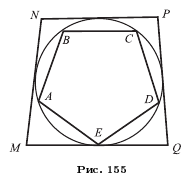
\includegraphics{mppics/ris-155}
\caption{}\label{1938/ris-155}
\end{wrapfigure}

Если все стороны какого-нибудь многоугольника ($MNPQ$, рис.~\ref{1938/ris-155}) касаются окружности, то говорят, что этот многоугольник \rindex{описанный многоугольник}\textbf{описан около окружности}, или что окружность \rindex{вписанная окружность}\textbf{вписана в него}.

\paragraph{}\label{1938/137}
\mbox{\so{Теоремы}.}
1) \textbf{\emph{Около всякого треугольника можно описать окружность и притом только одну.}}

2) \textbf{\emph{Во всякий треугольник можно вписать окружность и притом только одну.}}

1) Вершины $A$, $B$ и $C$ всякого треугольника суть три точки, не лежащие на одной прямой, а через такие точки, как мы видели (§~\ref{1938/104}), всегда можно провести окружность и притом только одну.

\begin{wrapfigure}{o}{40mm}
\centering
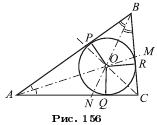
\includegraphics{mppics/ris-156}
\caption{}\label{1938/ris-156}
\end{wrapfigure}

2) Если возможна такая окружность, которая касалась бы всех сторон треугольника $ABC$ (рис.~\ref{1938/ris-156}),
то её центр должен быть точкой, одинаково удалённой от этих сторон.
Докажем, что такая точка существует.
Геометрическое место точек, равно отстоящих от сторон $AB$ и $AC$, есть биссектриса $AM$ угла $A$ (§~\ref{1938/60});
геометрическое место точек, равно отстоящих от сторон $BA$ и $BC$, есть биссектриса $BN$ угла $B$.
Эти две биссектрисы должны, очевидно, пересечься внутри треугольника в некоторой точке $O$.
Эта точка и будет равноудалённой от всех сторон треугольника, так как она находится на обоих геометрических местах.

Итак, чтобы вписать круг в треугольник, делим какие-нибудь два угла его, например $A$ и $B$, пополам и точку пересечения биссектрис берём за центр.
За радиус берём один из перпендикуляров $OP$, $OQ$ или $OR$, опущенных из центра на стороны треугольника.
Окружность коснётся сторон в точках $P$, $Q$ и $R$, так как стороны в этих точках перпендикулярны к радиусам в их концах, лежащих на окружности (§~\ref{1938/113}).
Другой вписанной окружности не может быть, так как две биссектрисы пересекаются только в одной точке, а из одной точки на прямую можно опустить только один перпендикуляр.

\smallskip
\so{Замечание}.
Оставляем самим учащимся убедиться, что центр описанной окружности лежит внутри треугольника только тогда, когда треугольник остроугольный;
в тупоугольном же треугольнике он лежит вне его, а в прямоугольном — на середине гипотенузы.
Центр вписанной окружности лежит всегда внутри треугольника.

\smallskip
\so{Следствие}.
Точка $O$ (рис.~\ref{1938/ris-156}), находясь на одинаковом расстоянии от сторон $CA$ и $CB$, должна лежать на биссектрисе угла $C$;
следовательно, \emph{биссектрисы трёх углов треугольника пересекаются в одной точке.}

\begin{wrapfigure}{r}{45mm}
\vskip-4mm
\centering
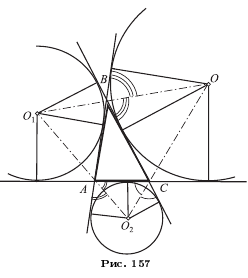
\includegraphics{mppics/ris-157}
\caption{}\label{1938/ris-157}
\end{wrapfigure}

\paragraph{Вневписанные окружности.}\label{1938/138}
Вневписанными называются окружности (рис.~\ref{1938/ris-157}), которые касаются одной стороны треугольника и \so{продолжений} двух других сторон (они лежат вне треугольника, вследствие чего и получили название \rindex{вневписанная окружность}\textbf{вневписанных}).


Таких окружностей для всякого треугольника может быть три.
Чтобы построить их, проводят биссектрисы внешних углов треугольника $ABC$ и точки их пересечений берут за центры.
Так, центром окружности, вписанной в угол $A$, служит точка $O_a$, то есть
пересечение биссектрис $BO_a$ и $CO_a$ внешних углов, не смежных с $A$;
радиус этой окружности есть перпендикуляр, опущенный из $O_a$ на какую-либо сторону треугольника.

\paragraph{Свойства вписанного выпуклого четырехугольника.}\label{1938/139}
1) \textbf{\emph{В выпуклом вписанном четырёхугольнике сумма противоположных углов равна $\bm{180\degree}$.}}

2) \textbf{\emph{Обратно, если в выпуклом четырёхугольнике сумма противоположных углов равна $180\degree$, то около него можно описать окружность.}}

\begin{wrapfigure}{o}{27mm}
\centering
\includegraphics{mppics/ris-158}
\caption{}\label{1938/ris-158}
\end{wrapfigure}

1) Пусть $ABCD$ (рис.~\ref{1938/ris-158}) есть вписанный выпуклый четырёхугольник;
требуется доказать, что
\[\angle B+\angle D = 180\degree
\quad\text{и}\quad 
\angle A + \angle C = 180\degree.\]

Так как сумма всех четырёх углов всякого выпуклого четырёхугольника равна $360\degree$ (§~\ref{1938/82}), то достаточно доказать только одно из требуемых равенств.

Докажем, например, что $\angle B+\angle D = 180\degree$.

Углы $B$ и $D$, как вписанные, измеряются:
первый — половиной дуги $ADC$, второй — половиной дуги $ABC$;
следовательно, сумма $\angle B+\angle D$ измеряется суммой $\tfrac12{\smallsmile}ADC + \tfrac12{\smallsmile}ABC$, а эта сумма равна $\tfrac12({\smallsmile}ADC+{\smallsmile}ABC)$, то есть
равна половине окружности;
значит:
\[\angle B+\angle D=180\degree.\]

2) Пусть $ABCD$ (рис.~\ref{1938/ris-158}) есть такой выпуклый четырёхугольник, у которого $\angle B+\angle D = 180\degree$, и, следовательно, $\angle A \z+ \angle C =180\degree$.
Требуется доказать, что около такого четырёхугольника можно описать окружность.

Через какие-нибудь три его вершины, например через $A$, $B$ и $C$, проведём окружность (что всегда можно сделать).
Четвёртая вершина $D$ должна находиться на этой окружности, потому что в противном случае вершина угла $B$ лежала бы или внутри круга, или вне его, и тогда этот угол не измерялся бы половиной дуги $ABC$;
поэтому сумма $\angle B+\angle D$ не измерялась бы полусуммой дуг $ADC$ а $ABC$ (§~\ref{1938/130}) и, значит, сумма $\angle B+\angle D$ не равнялась бы $180\degree$, что противоречит условию.

\smallskip
\so{Следствия}.
1) \emph{Из всех параллелограммов только около прямоугольника можно описать окружность.}

2) \emph{Около трапеции можно описать окружность только тогда, когда она равнобочная.}

\paragraph{Свойство описанного четырехугольника.}\label{1938/140}
\textbf{\emph{В описанном четырёхугольнике суммы противоположных сторон равны.}}

Пусть $ABCD$ (рис.~\ref{1938/ris-159}) будет описанный четырёхугольник, то есть стороны его касаются окружности;
требуется доказать, что 
\[AB+CD=BC+AD.\]

\begin{wrapfigure}{o}{44mm}
\centering
\includegraphics{mppics/ris-159}
\caption{}\label{1938/ris-159}
\end{wrapfigure}

Обозначим точки касания буквами $M$, $N$, $P$ и $Q$.
Так как две касательные, проведённые из одной точки к окружности, равны, то 
\begin{align*}
AM&=AQ,& BM&=BN,
\\
CP&=CN, & DP &= DQ.
\end{align*}

Следовательно,
\begin{align*}
AM&+MB+CP+PD = 
\\
&=AQ + QD+BN+NC,
\end{align*}
то есть 
\[AB+CD=AD+BC.\]
